\documentclass[compress]{beamer}
\usecolortheme{default}

\usepackage{lmodern, epstopdf, multirow, array, setspace, bbm, tcolorbox, pbox, bm, mathtools, tikz}
\usepackage[T1]{fontenc}

\setbeamertemplate{frametitle}[default][center]
\setbeamertemplate{footline}{\hfill \insertframenumber/\inserttotalframenumber\hspace*{5pt}\vspace{5pt}}
\setbeamertemplate{navigation symbols}{}

\newlength{\wideitemsep}
\setlength{\wideitemsep}{\itemsep}
\addtolength{\wideitemsep}{4pt}
\let\olditem\item
\renewcommand{\item}{\setlength{\itemsep}{\wideitemsep}\olditem}
\setlength{\leftmargini}{12pt}
\setlength{\leftmarginii}{14pt}
\setbeamertemplate{itemize/enumerate subbody begin}{\vspace{6pt}}
\setbeamertemplate{itemize item}[circle]
\setbeamertemplate{enumerate item}[circle]
\setbeamertemplate{enumerate subitem}[default]

\setbeamercolor{alerted text}{fg=blue}
\setbeamersize{text margin left=1.5em,text margin right=1.5em}

\tcbset{
    colback=white,
    colframe=black,
    coltext=black,
    coltitle=blue,
    colbacktitle=white,
    boxrule=1pt,
    titlerule=0pt,
    toptitle=4pt,
    top=2pt
}

\newenvironment{changemargin}[2]{% 
  \begin{list}{}{% 
    \setlength{\topsep}{0pt}% 
    \setlength{\leftmargin}{#1}% 
    \setlength{\rightmargin}{#2}% 
    \setlength{\listparindent}{\parindent}% 
    \setlength{\itemindent}{\parindent}% 
    \setlength{\parsep}{\parskip}% 
  }% 
  \item[]}{\end{list}}
  
\newenvironment{defn}{%
  \begin{tcolorbox}[title={Definition}]%
  }{\end{tcolorbox}}
  
\newenvironment{prop}[1]{%
  \begin{tcolorbox}[title={Proposition #1}]%
  }{\end{tcolorbox}}
  
\newcommand{\cit}[1]{{\footnotesize \textcolor[rgb]{0.5,0,0}{#1}}}

% Font size for code listings (verbatim blocks); reset with \normalsize
\newcommand{\codesize}{\fontsize{7}{8.5}\selectfont}

\newcommand{\slidesetup}[1]{%
  \title{#1}%
  \subtitle{\texorpdfstring{\vspace{0.3\baselineskip}}{} {\small This version: \today}}%
  \author[Mikkel Plagborg-Moller]{ECMA 31150, Spring 2026 \texorpdfstring{\\[0.5ex]}{} University of Chicago \texorpdfstring{\\[0.5ex]}{} Department of Economics \texorpdfstring{\\[4ex]}{} Mikkel Plagborg-Moller}%
  \date{}%
}

% \circleoverlay[options]{text}
% Draws a red circle with a text box nearby on a tikz overlay.
% Options (with defaults):
%   cx=0cm, cy=0cm      - circle center (shift from page center)
%   r=1cm               - circle radius
%   tx=0cm, ty=0cm      - text box offset from circle center
%   text anchor=east    - anchor of text node (east = text left, west = text right)
%   font=\normalsize    - font size for text
\pgfkeys{
  /circleoverlay/.cd,
  cx/.store in=\cocx, cx=0cm,
  cy/.store in=\cocy, cy=0cm,
  r/.store in=\cor, r=1cm,
  tx/.store in=\cotx, tx=0cm,
  ty/.store in=\coty, ty=0cm,
  text anchor/.store in=\cotextanchor, text anchor=east,
  font/.store in=\cofont, font=\normalsize,
}
\newcommand{\circleoverlay}[2][]{%
  \pgfkeys{/circleoverlay/.cd, cx=0cm, cy=0cm, r=1cm, tx=0cm, ty=0cm, text anchor=east, font=\normalsize, #1}%
  \pgfmathsetlengthmacro{\circlediameter}{2*\cor}%
  \node[draw=red, line width=2pt, circle, minimum size=\circlediameter, inner sep=0pt]
    (tmpcirc) at ([xshift=\cocx,yshift=\cocy]current page.center) {};%
  \node[anchor=\cotextanchor, fill=white, draw=red, text=red, inner sep=4pt, align=left, font=\cofont]
    at ([xshift=\cotx,yshift=\coty]tmpcirc.center) {#2};%
}

\DeclareMathOperator*{\argmax}{argmax}
\DeclareMathOperator*{\argmin}{argmin}
\DeclareMathOperator{\diag}{diag}
\DeclareMathOperator{\var}{Var}
\DeclareMathOperator{\cov}{Cov}
\DeclareMathOperator{\corr}{Corr}
\DeclareMathOperator{\lrv}{LRV}


\slidesetup{Non-stationary models II}

\begin{document}
\frame{
\maketitle
}

\frame{
\frametitle{Plan for this slide deck}
\begin{enumerate}
\item Regressions involving two trending variables
\item Modeling multiple time series with common trends
\item Testing for structural breaks
\item Removing trends and seasonality from data
\end{enumerate}
}

\frame{
\frametitle{Spurious regression}
\begin{itemize}
\item Assume the two series $\lbrace y_t \rbrace$ and $\lbrace x_t \rbrace$ are driftless random walks that are completely independent of each other.
\item Suppose we nevertheless run an OLS regression (without lags):
\[y_t = \hat{c} + \hat{\beta} x_t + \hat{v}_t.\]
\item Then $\hat{\beta}$ does not converge to 0, and the magnitude of the t-statistic for testing $\beta=0$ diverges to $\infty$ as $T \to \infty$!
\begin{itemize}
\item The $R^2$ value converges to a non-degenerate random variable in $[0,1]$.
\end{itemize}
\item \textbf{Spurious regression:} a regression of two independent trending series on each other can spuriously indicate a significant relationship if we interpret the OLS output naively.
\begin{itemize}
\item Intuitively, the stochastic trends in the series act as ``omitted variables''.
\end{itemize}
\end{itemize}
}

\frame{
\begin{figure}
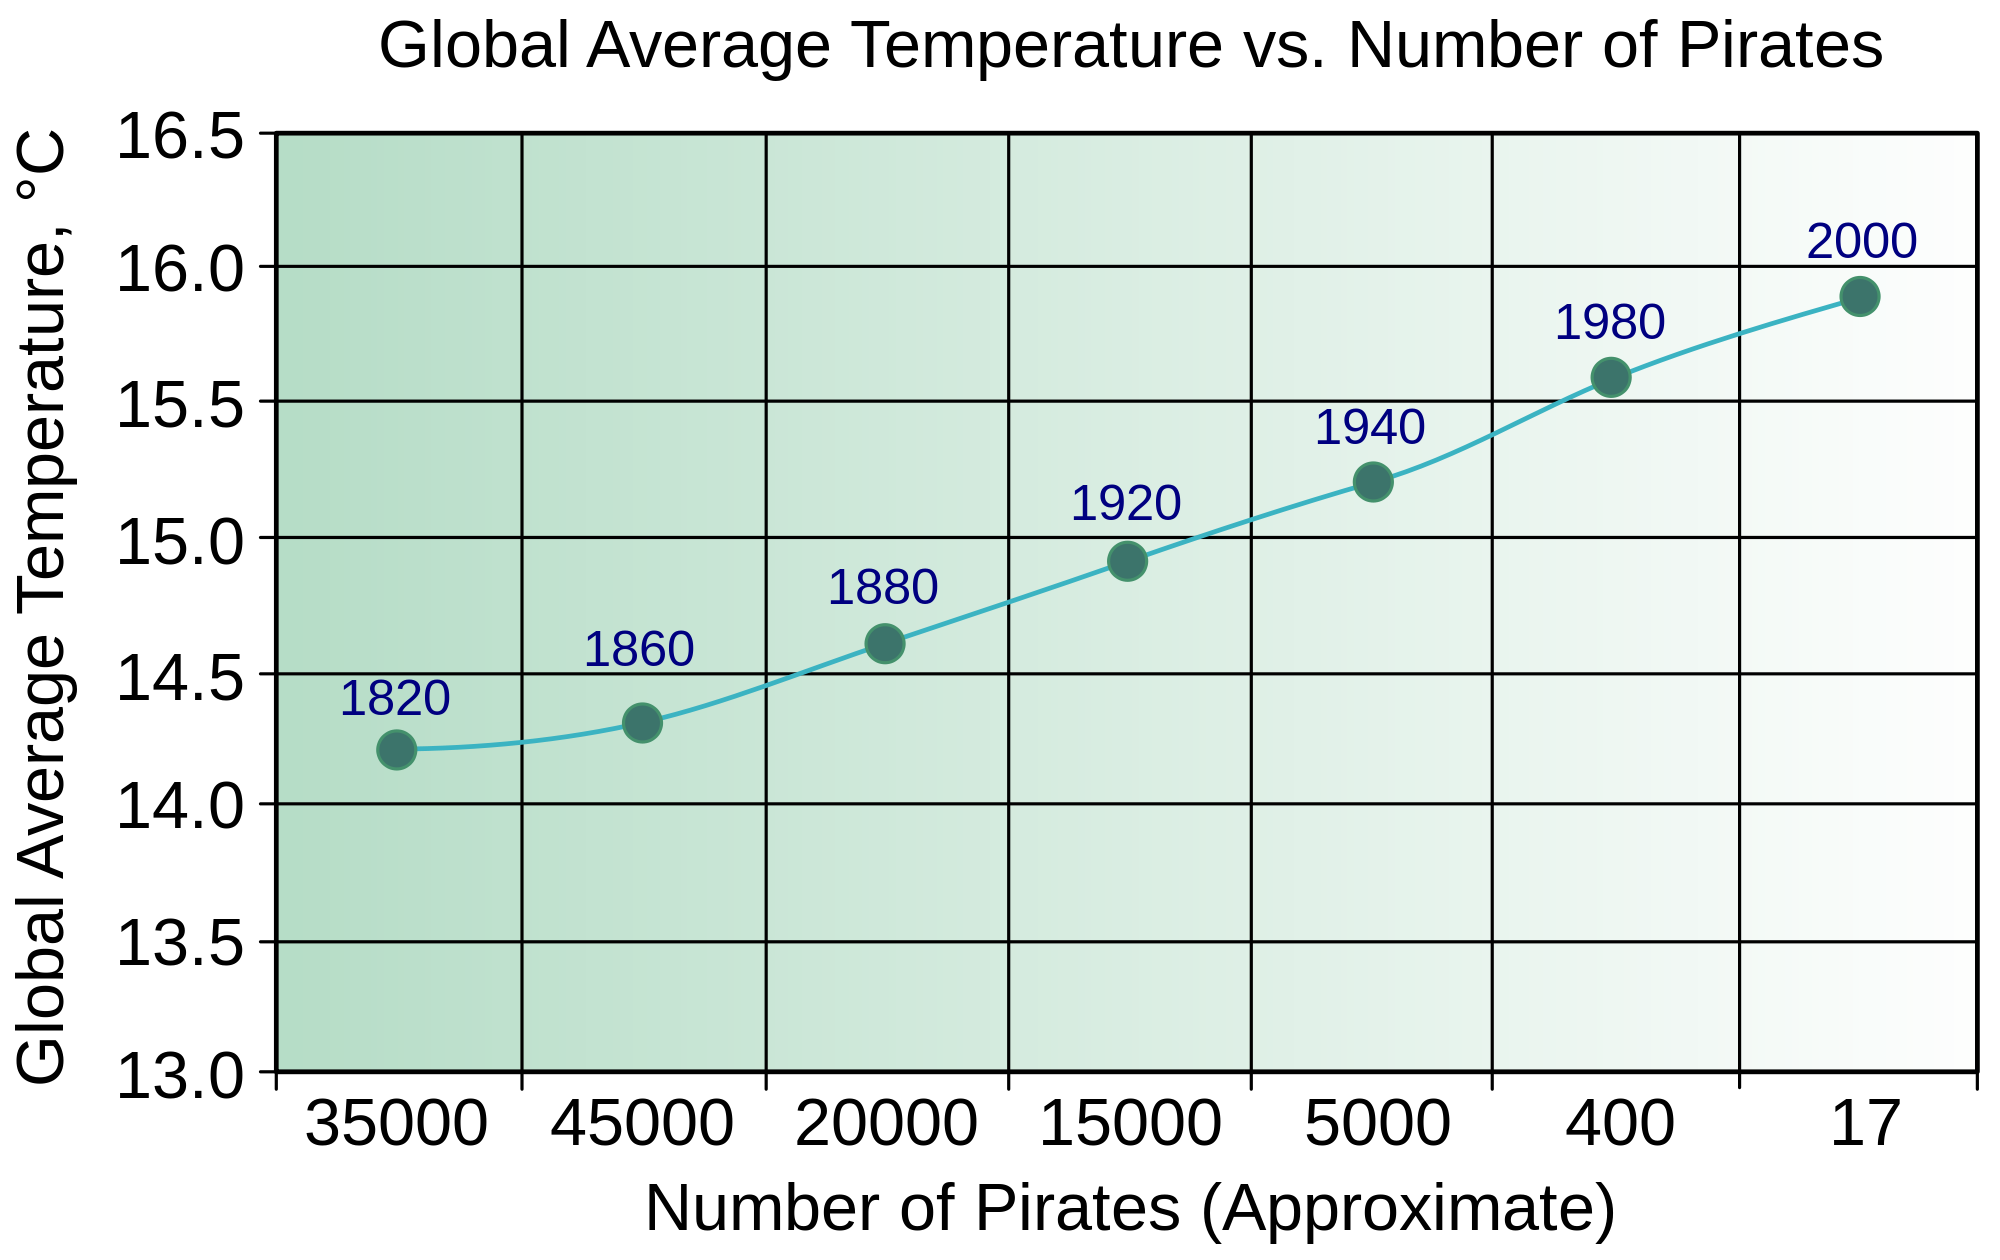
\includegraphics[width=\linewidth]{fig/PiratesVsTemp.png} \\
\medskip
\scriptsize Source: \url{https://commons.wikimedia.org/wiki/File:PiratesVsTemp(en).svg}
\end{figure}
}

\frame{
\frametitle{Common stochastic trends}
\begin{itemize}
\item Since regressions using variables with \emph{independent} trends can be spurious, we need a framework for evaluating whether trends are independent or shared.
\item Let's consider the case where the two I(1) series $y_t$ and $x_t$ share the \emph{same} stochastic trend:
\begin{align*}
y_t &= \lambda_1 \alert{w_t} + v_{yt}, \\
x_t &= \lambda_2 \alert{w_t} + v_{xt},
\end{align*}
where $w_t$ is an I(1) series and $(v_{yt},v_{xt})$ are covariance stationary.
\end{itemize}
}

\frame{
\frametitle{Cointegration}
\begin{align*}
y_t &= \lambda_1 w_t + v_{yt}, \\
x_t &= \lambda_2 w_t + v_{xt},
\end{align*}
\vspace{-\baselineskip}
\begin{itemize}
\item Though each of $y_t$ and $x_t$ is non-stationary, a \emph{linear combination} of them is covariance stationary:
\[y_t - \frac{\lambda_1}{\lambda_2} x_t = \underbrace{\left(\lambda_1 - \frac{\lambda_1}{\lambda_2} \lambda_2\right)}_{=0}w_t + \underbrace{v_{yt} - \frac{\lambda_1}{\lambda_2} v_{xt}}_\text{cov.\ stationary}.\]
(Any scalar multiple of this linear combination also works.)
\item $(y_t,x_t)$ are \textbf{cointegrated}: they have a stable long-run relationship.
\end{itemize}
}

\frame{
\begin{figure}
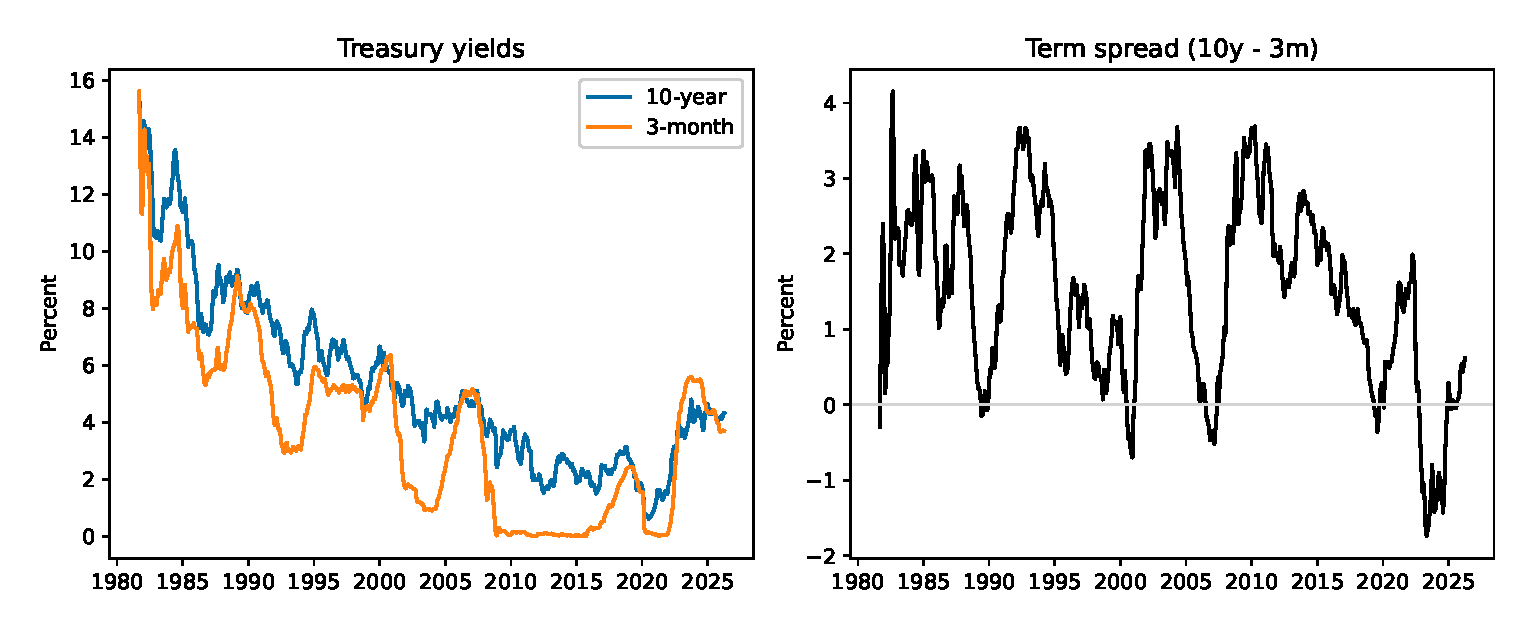
\includegraphics[width=\linewidth]{fig/treasury_yields.eps} \\
\bigskip
The spread $y_{\text{10y},t}-y_{\text{3m},t}$ looks roughly stationary, \\
even though each individual yield is trending
\end{figure}
}

\frame{
\frametitle{Testing for a known cointegrating relationship}
\begin{itemize}
\item Consider two trending series $y_t$ and $x_t$. They may share a common stochastic trend (cointegration) or each follow their own trend.
\item Suppose we want to test for cointegration with a \emph{known} cointegrating relationship $y_t-\beta x_t$.
\begin{itemize}
\item E.g., $\beta=1$ for the yield spread on the previous slide.
\end{itemize}
\item First we run two ADF tests to test whether each of $y_t$ and $x_t$ is individually I(1).
\begin{itemize}
\item If we reject the null of a unit root for either, then they obviously can't share a common stochastic trend.
\end{itemize}
\item Then we run another ADF test on the purported cointegrating relationship $y_t-\beta x_t$. If we reject a unit root, then we reject the null hypothesis that the series are \emph{not} cointegrated.
\end{itemize}
}

\begin{frame}[fragile]
\scriptsize
\begin{verbatim}
# ADF unit root test for each series (constant + trend)
for s in ['GS3M', 'GS10']:
    stat, pval, nlags, *_ = adfuller(df[s], regression='ct', autolag='AIC')
    print(f'{s}: ADF stat = {stat:.3f}, p-value = {pval:.3f}, lags = {nlags}')

# Test known cointegrating relationship (no trend)
stat, pval, nlags, *_ = adfuller(df['spread'], regression='c', autolag='AIC')
print(f'Spread: ADF stat = {stat:.3f}, p-value = {pval:.3f}, lags = {nlags}')
\end{verbatim}
\normalsize \bigskip
\textbf{Results:}
\smallskip \scriptsize
\begin{verbatim}
GS3M: ADF stat = -2.856, p-value = 0.177, lags = 10
GS10: ADF stat = -2.971, p-value = 0.140, lags = 3
Spread: ADF stat = -3.874, p-value = 0.002, lags = 9
\end{verbatim}
\normalsize \bigskip
We fail to reject the null that each series is individually I(1). We do reject the null of no cointegration. (5\% significance level.)
\end{frame}

\frame{
\frametitle{Estimating cointegrating relationships}
\begin{itemize}
\item If two series $y_t$ and $x_t$ are cointegrated, we can estimate the cointegrating relationship consistently by running an OLS regression:
\[y_t = \hat{c} + \hat{\beta}x_t + \hat{v}_t.\]
The estimated cointegrating relationship is $y_t-\hat{\beta} x_t$.
\item $\hat{\beta}$ is consistent under cointegration (in fact, super-consistent).
\item However, because of the stochastic trend, the OLS estimator $\hat{\beta}$ is non-normally distributed, so we cannot rely on the usual t-test or confidence interval.
\begin{itemize}
\item There exist other estimation approaches that have a normal limiting distribution. See Stock \& Watson textbook, chapter 17.4.
\end{itemize}
\end{itemize}
}

\begin{frame}[fragile]
\scriptsize
\begin{verbatim}
                            OLS Regression Results                            
==============================================================================
Dep. Variable:                   GS10   R-squared:                       0.845
Model:                            OLS   Adj. R-squared:                  0.845
Method:                 Least Squares   F-statistic:                     2914.
Date:                Wed, 20 May 2026   Prob (F-statistic):          2.05e-218
Time:                        15:30:39   Log-Likelihood:                -859.91
No. Observations:                 536   AIC:                             1724.
Df Residuals:                     534   BIC:                             1732.
Df Model:                           1                                         
Covariance Type:            nonrobust                                         
==============================================================================
                 coef    std err          t      P>|t|      [0.025      0.975]
------------------------------------------------------------------------------
const          1.9185      0.082     23.267      0.000       1.757       2.081
GS3M           0.9007      0.017     53.977      0.000       0.868       0.933
==============================================================================
\end{verbatim}
\normalsize
Recall: t-test and conf.\ interval are invalid, as they rely on normality
\end{frame}

\frame{
\frametitle{Testing for an unknown cointegrating relationship}
\begin{itemize}
\item To test whether $y_t$ and $x_t$ are cointegrated with an \emph{unknown} cointegrating relationship:
\begin{enumerate}
\item Estimate the cointegrating relationship by an OLS regression of $y_t$ on $x_t$ (as on previous slide).
\item Run an ADF test on $y_t-\hat{\beta} x_t$. If it rejects a unit root, then we reject the null of no cointegration.
\end{enumerate}
\item However, it turns out that the estimation error in $\hat{\beta}$ changes the limiting distribution of the ADF t-statistic. So the critical values for the second step must be adjusted relative to the case with known $\beta$.
\item This \textbf{Engle \& Granger ADF} (EG-ADF) test with corrected critical values is built into many software packages.
\end{itemize}
}

\begin{frame}[fragile]
\scriptsize
\begin{verbatim}
# EG-ADF test with estimated cointegrating relationship
stat, pval, _ = coint(df['GS10'], df['GS3M'], trend='c', autolag='AIC')
print(f'EG-ADF stat = {stat:.3f}, p-value = {pval:.3f}')
\end{verbatim}
\normalsize \bigskip
\textbf{Results:}
\smallskip \scriptsize
\begin{verbatim}
EG-ADF stat = -3.450, p-value = 0.037
\end{verbatim}
\normalsize \bigskip
We reject the null of no cointegration at the 5\% level.
\end{frame}

\frame{
\frametitle{Error correction model}
\begin{itemize}
\item If $y_t$ and $x_t$ are cointegrated, then changes in these series should be predictable by the cointegrating relationship:
\begin{align*}
\Delta y_t &= c_y + A_{yy} \Delta y_{t-1} + A_{yx} \Delta x_{t-1} + A_{yc} (\alert{y_{t-1}-\beta x_{t-1}}) + u_{yt}, \\
\Delta x_t &= c_x + A_{xy} \Delta y_{t-1} + A_{xx} \Delta x_{t-1} + A_{xc} (\alert{y_{t-1}-\beta x_{t-1}}) + u_{xt}.
\end{align*}
\item \textbf{Error correction model}: if $y_t$ is currently far away from $\beta x_t$, then we expect these to move closer together in the future, because their difference is covariance stationary.
\item If we naively run a VAR in the first differences ($\Delta y_t,\Delta x_t$), we lose out on the predictive power of the cointegrating relationship (a.k.a.\ error correction term).
\item Running a VAR in the levels $(y_t,x_t)$ is more robust as it allows for cointegrating relationships among the variables.
\end{itemize}
}

\frame{
\frametitle{Regression with trending variables: summary}
\begin{itemize}
\item We should be careful with regressions involving trending variables.
\item If we have theoretical reasons to expect cointegration (shared trend), we could test for it or impose a known cointegrating relationship directly in an error correction model.
\item For many purposes it suffices to just run a VAR (or LP) with a generous number of lags. The lags solve the spurious regression problem.
\item The cointegration concept can be extended to relationships involving more than two variables. See Stock \& Watson textbook, chapter 17.4.
\end{itemize}
}

\frame{
\frametitle{Structural breaks}
\begin{itemize}
\item \textbf{Structural breaks}: changes in the data generating process over time. Different kind of non-stationarity from trends.
\item We've already discussed how to use state space models to analyze time-variation in parameters that is (a) \emph{gradual and period-by-period} or (b) \emph{discrete and intermittent}.
\item In some applications, we might instead expect that the parameters have undergone a \emph{large, one-time} break.
\item Let's consider the regression example:
\[y_t = c + \beta_t x_t + v_t,\quad \beta_t = \begin{cases}
\beta & \text{for } t < t^*, \\
\beta + \delta & \text{for } t \geq t^*,
\end{cases}\]
where $t^*$ is the break date and $\delta \neq 0$ is the break magnitude.
\end{itemize}
}

\frame{
\frametitle{Testing for break at a known date}
\begin{itemize}
\item If the potential break date $t^*$ is \emph{known} to us, we can test for breaks using a \textbf{Chow test}:
\begin{enumerate}
\item Define the break indicator
\[d_t \equiv \begin{cases}
0 & \text{for } t<t^*, \\
1 & \text{for } t\geq t^*.
\end{cases}\]
\item Run an OLS regression with interaction term:
\[y_t = \hat{c} + \hat{\beta} x_t + \hat{\delta} (x_t \times d_t) + \hat{v}_t.\]
\item Test the null hypothesis $\delta=0$ (no break) with a t-test.
\end{enumerate}
\item More generally, if we want to test for breaks in coefficients on multiple covariates, we include interactions of $d_t$ with each of those. Then do an F-test for the joint significance of the coefficients on the interaction terms.
\end{itemize}
}

\begin{frame}[fragile]
\codesize
\begin{verbatim}
# Load data
gdp = pd.read_csv('data/GDPC1.csv', index_col='observation_date',
  parse_dates=True)
spread = pd.read_csv('data/T10Y3MM.csv', index_col='observation_date',
  parse_dates=True)

gdp['gdp_growth'] = 400 * np.log(gdp['GDPC1']).diff()
spread_q = spread.resample('QS').mean()

df_adl = gdp[['gdp_growth']].join(spread_q, how='inner')
df_adl = df_adl.loc[:'2019'] # pre-2020 sample

# Full-sample ADL regression
df_adl['gdp_growth_lag1'] = df_adl['gdp_growth'].shift(1)
df_adl['gdp_growth_lag2'] = df_adl['gdp_growth'].shift(2)
df_adl['spread_lag1']     = df_adl['T10Y3MM'].shift(1)
df_adl['spread_lag2']     = df_adl['T10Y3MM'].shift(2)

covariates = ['gdp_growth_lag1', 'gdp_growth_lag2', 'spread_lag1', 'spread_lag2']
X_adl = sm.add_constant(df_adl[covariates])
res_adl = sm.OLS(df_adl['gdp_growth'], X_adl, missing='drop').fit(cov_type='HC1')
print(res_adl.summary())
\end{verbatim}
\end{frame}

\begin{frame}[fragile]
\codesize
\begin{verbatim}
                            OLS Regression Results                            
==============================================================================
Dep. Variable:             gdp_growth   R-squared:                       0.260
Model:                            OLS   Adj. R-squared:                  0.239
Method:                 Least Squares   F-statistic:                     11.49
Date:                Wed, 20 May 2026   Prob (F-statistic):           3.94e-08
Time:                        15:30:39   Log-Likelihood:                -322.65
No. Observations:                 150   AIC:                             655.3
Df Residuals:                     145   BIC:                             670.4
Df Model:                           4                                         
Covariance Type:                  HC1                                         
===================================================================================
                      coef    std err          z      P>|z|      [0.025      0.975]
-----------------------------------------------------------------------------------
const               0.9231      0.409      2.259      0.024       0.122       1.724
gdp_growth_lag1     0.3438      0.105      3.280      0.001       0.138       0.549
gdp_growth_lag2     0.2128      0.080      2.652      0.008       0.056       0.370
spread_lag1        -0.2585      0.304     -0.849      0.396      -0.855       0.338
spread_lag2         0.4460      0.329      1.355      0.175      -0.199       1.091
==============================================================================

Notes:
[1] Standard Errors are heteroscedasticity robust (HC1)
\end{verbatim}
\end{frame}

\begin{frame}[fragile]
\scriptsize
\begin{verbatim}
def chow_test(break_date):
    brk = (df_adl.index >= break_date).astype(float)
    breaks = pd.DataFrame({
        'break_spread_lag1': brk * df_adl['spread_lag1'],
        'break_spread_lag2': brk * df_adl['spread_lag2'],
    })
    X = sm.add_constant(pd.concat([df_adl[covariates], breaks], axis=1))
    res = sm.OLS(df_adl['gdp_growth'], X, missing='drop').fit(cov_type='HC1')
    f_test = res.f_test('break_spread_lag1 = break_spread_lag2 = 0')
    return res, f_test

# Chow test for 2008q3
res_chow, f_chow = chow_test('2008-07-01')
print(res_chow.summary())
print('\nChow test')
print(f_chow)
\end{verbatim}
\bigskip \normalsize
Note: here we're only testing for breaks in the coefficients on the lagged spread (not lagged GDP growth or the intercept)
\end{frame}

\begin{frame}[fragile]
\codesize
\begin{verbatim}
                            OLS Regression Results                            
==============================================================================
Dep. Variable:             gdp_growth   R-squared:                       0.286
Model:                            OLS   Adj. R-squared:                  0.256
Method:                 Least Squares   F-statistic:                     8.387
Date:                Wed, 20 May 2026   Prob (F-statistic):           8.47e-08
Time:                        15:30:39   Log-Likelihood:                -319.96
No. Observations:                 150   AIC:                             653.9
Df Residuals:                     143   BIC:                             675.0
Df Model:                           6                                         
Covariance Type:                  HC1                                         
=====================================================================================
                        coef    std err          z      P>|z|      [0.025      0.975]
-------------------------------------------------------------------------------------
const                 1.1067      0.420      2.634      0.008       0.283       1.930
gdp_growth_lag1       0.3002      0.099      3.027      0.002       0.106       0.494
gdp_growth_lag2       0.1818      0.087      2.096      0.036       0.012       0.352
spread_lag1          -0.1262      0.334     -0.378      0.706      -0.782       0.529
spread_lag2           0.4610      0.364      1.266      0.206      -0.253       1.175
break_spread_lag1    -1.0399      0.939     -1.108      0.268      -2.880       0.800
break_spread_lag2     0.6386      0.892      0.716      0.474      -1.111       2.388
==============================================================================

Notes:
[1] Standard Errors are heteroscedasticity robust (HC1)

Chow test
<F test: F=2.209285321811282, p=0.11351275499888673, df_denom=143, df_num=2>
\end{verbatim}
\uncover<2>{%
\begin{tikzpicture}[overlay, remember picture]
  \circleoverlay[cx=-1.5cm, cy=-3.65cm, r=0.5cm,
                 tx=0.8cm, ty=0.8cm, text anchor=west]{Fail to reject \\ null of no break}
\end{tikzpicture}
}
\end{frame}

\frame{
\frametitle{Testing for break at an unknown date}
\begin{itemize}
\item Often we don't know the exact break date $t^*$ \emph{a priori}.
\item Instead, we can run a Chow test for \emph{every possible} candidate break date $t^*$ in some range and record the \textbf{largest} F-statistic. This is called the \textbf{Quandt likelihood ratio} (QLR) statistic.
\begin{itemize}
\item To avoid small-sample issues near the boundaries, it's common to restrict the candidate break dates to the central 70\% of the sample.
\end{itemize}
\item We can't compare the QLR-stat with the usual critical value for an F-test because of the \textbf{multiple testing} problem: we're implicitly testing for the null of no break at very many time points. The probability of type-I error compounds across tests.
\item Critical values for the QLR test that adjust for multiple testing can be found in Stock \& Watson, chapter 15.8.
\end{itemize}
}

\begin{frame}[fragile]
\footnotesize
\begin{verbatim}
# QLR test
sample = X_adl.dropna().index
trim = 0.15
i_lo = int(np.ceil(trim * len(sample)))
i_hi = int(np.floor((1 - trim) * len(sample)))
break_dates = sample[i_lo:i_hi] # central 70% of sample

f_stats = pd.Series(index=break_dates, dtype=float)
for t in break_dates:
    _, f_test = chow_test(t)
    f_stats[t] = f_test.statistic
\end{verbatim}
\end{frame}

\frame{
\begin{figure}
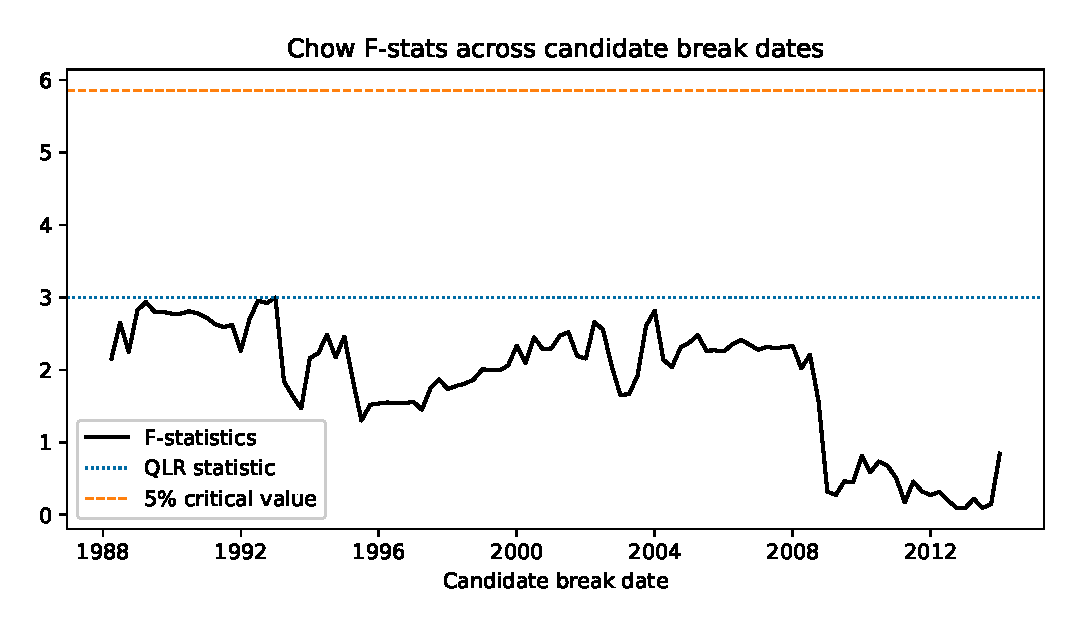
\includegraphics[width=\linewidth]{fig/qlr.eps} \\
\medskip
QLR critical value = 5.86 (for 2 restrictions, 15\% sample trimming at each end, 5\% significance level) \\
\medskip
Here we fail to reject the null hypothesis of no breaks
\end{figure}
}

\frame{
\frametitle{Estimated break date, multiple breaks}
\begin{itemize}
\item If the QLR test detects a break, the time point $t^*$ yielding the largest F-stat is an estimator of the break date.
\begin{itemize}
\item For subsequent analysis, we can estimate our model separately on each subsample $t \in [1,t^*-1]$ and $t \in [t^*,T]$.
\end{itemize}
\item If we suspect multiple large breaks, we can apply the QLR test again on the subsamples.
\item The QLR test usually also has decent power against the alternative hypothesis of gradual time-variation (as opposed to one large break), though in this case the estimated break date is meaningless.
\end{itemize}
}

\frame{
\frametitle{Seasonality}
\begin{itemize}
\item Some time series exhibit \textbf{seasonality}: they behave systematically differently at some points of the year than at others.
\begin{itemize}
\item For example, due to holidays or annual temperature cycles.
\end{itemize}
\item This is yet another form of non-stationarity.
\item We can try to control for seasonal effects by including dummy variables for each within-year ``season'' in our regressions.
\begin{itemize}
\item E.g., in quarterly data, control for 3 dummy variables for 1st, 2nd, and 3rd quarter of the year.
\end{itemize}
\item But usually best to just use \textbf{seasonally adjusted} data supplied by statistical agencies. They use more advanced techniques to remove seasonal patterns.
\end{itemize}
}

\frame{
\begin{figure}
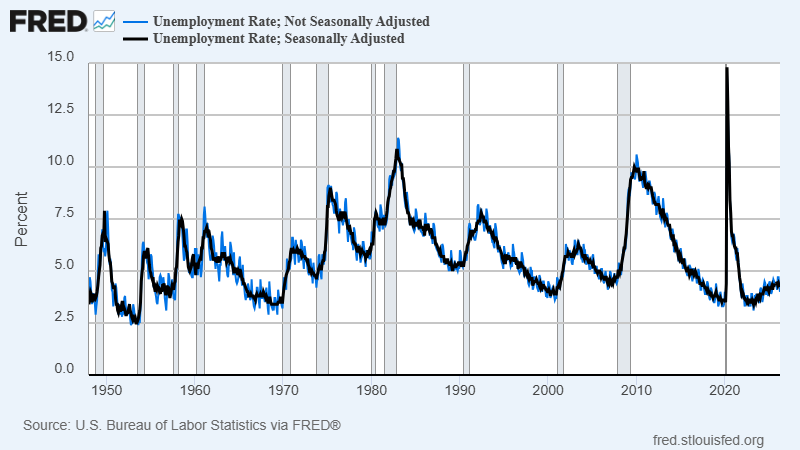
\includegraphics[width=\linewidth]{fig/fred_unrate_seas.png}
\end{figure}
}

\frame{
\frametitle{Detrending}
\begin{itemize}
\item When working with trending data, some papers choose to \textbf{detrend} their data prior to analysis.
\item The most common procedure is the \textbf{Hodrick-Prescott filter}, which fits a slow-moving trend to the data and then subtracts that estimated trend.
\item But the inevitable estimation error in the trend can impart spurious dynamics in the ``detrended'' residual.
\begin{itemize}
\item See Hamilton (2018) paper on the syllabus for discussion.
\end{itemize}
\item Detrending also removes any predictive power arising from cointegrating relationships.
\item Usually best to avoid detrending if possible and instead tackle stochastic trends directly, as we've discussed.
\end{itemize}
}

\frame{
\frametitle{What did we learn?}
\begin{itemize}
\item Spurious regression
\item Cointegration
\begin{itemize}
\item Known cointegrating relationship: ADF test
\item Unknown cointegrating relationship: EG-ADF test
\item Error correction model, naive differencing loses information
\end{itemize}
\item Testing for structural breaks
\begin{itemize}
\item Known break date: Chow test
\item Unknown break date: QLR test
\end{itemize}
\item Seasonality, detrending
\end{itemize}
}

\end{document}